\chapter{Konzept}
\label{chapter_Konzept}

Im folgenden Kapitel wird auf die Erstellung des Konzeptes eingegangen.

\section{Teststand}
\label{section_Teststand}

Das Gesamtsystem setzt sich aus drei Untersystemen zusammen:

\begin{itemize}

\item Mess-Slave
\begin{itemize}
\item Übernimmt die lokale Ansteuerung der \acp{DUT}
\item Nimmt Messdaten auf und stellt sie zur Verfügung
\end{itemize}

\item Mess-Master
\begin{itemize}
\item Verwaltet angeschlossene Mess-Slaves
\item Speichert alle Messdaten
\item Bildet das Bindeglied zwischen Mess-Slave und dem PC
\end{itemize}

\item PC Verwaltung
\begin{itemize}
\item Parametriert die Mess-Slaves
\item Wertet Messdaten aus und stellt sie leserlich da
\end{itemize}

\end{itemize}
\subsection{Mess-Slave}
\label{section_Mess-Slave}

Das Herzstück des Mess-Slave bildet ein STM8  8-Bit Mikrocontroller der Firma STMicroelectronics.
Auf jedem Mess-Slave sind 64 \acp{DUT} befestigt. In zyklischen Abständen werden die Messdaten der Prüfobjekte aufgenommen und über eine RS232-Schnittstelle zur Verfügung gestellt (siehe Abbildung \ref{MessSlaveBlockPlan}.\\
Dieses System war zum großen Teil bereits gegeben, so dass lediglich die Übertragung der RS232 Schnittstelle geregelt werden musste. Dazu wurde ein Protokoll für die Kommunikation entworfen (sieht Abschnitt \ref{section_RS232_Protokoll}).
\\
%\begin{figure}[h]
%\begin{center}
%\includegraphics[width=\textwidth]{}
%\caption{Mess-Slave Blockschaltplan}
%\label{MessSlaveBlockPlan}
%\end{center}
%\end{figure}


\subsection{Mess-Master}
\label{section_Mess-Master}

Als Mess-Master wird ein BeagleBone Black von Texas Instruments eingesetzt. Dabei handelt es sich um einen Einplatinen-Computer, der mit einem AM335x 1GHz ARM® Cortex-A8 Prozessor arbeitet. Das Betriebssystem ist eine Embedded Linux Debian Lösung.


\subsection{PC Verwaltung}
\label{section_Verwaltung}
asdasad


\subsection{RS232 Protokoll}
\label{section_RS232_Protokoll}
Das Protokoll für die Kommunikation über die RS232 Schnittstelle ist nötig, um die Validität, Vollständigkeit und Zuverlässigkeit der Übertragungen sicherzustellen.\ \\

Folgende Kriterien sollen dabei gegeben sein:
\begin{itemize}
\item Adressierung individueller Kommunikationspartner
\item Senden verschiedener Befehle
\item Variable Größe der Daten
\item Sicherstellung der Validität des Rahmens
\end{itemize}
\ \\
Daraus ergibt sich folgendes Protokoll.

\section{Datenbank}
\label{section_EntwurfDatenbank}

Die Datenbank muss folgende Daten für die Parameter der Mess-Slaves aufnehmen:\\

\begin{table}[h]
\centering
\begin{tabular}{|l|l|}\hline
Parameter & Beschreibung \\ \hline
DAC & Vorverstärker Wert\\ 
duration\_int1 & Dauer der Zeit die Werte im 1.Interval aufgenommen werden in Tagen\\ 
duration\_int2 & Dauer der Zeit die Werte im 2.Interval aufgenommen werden in Tagen\\ 
interval\_1 & Abstand zwischen den Messungen im 1. Interval in Minuten\\ 
interval\_2 & Abstand zwischen den Messungen im 2. Interval in Minuten\\ 
interval\_3 & Abstand zwischen den Messungen nach dem 2. Interval in Minuten\\ \hline
\end{tabular}
\caption{Parameter Tabelle}
\label{table_Parameter}
\end{table}

\begin{figure}[h]
\begin{center}
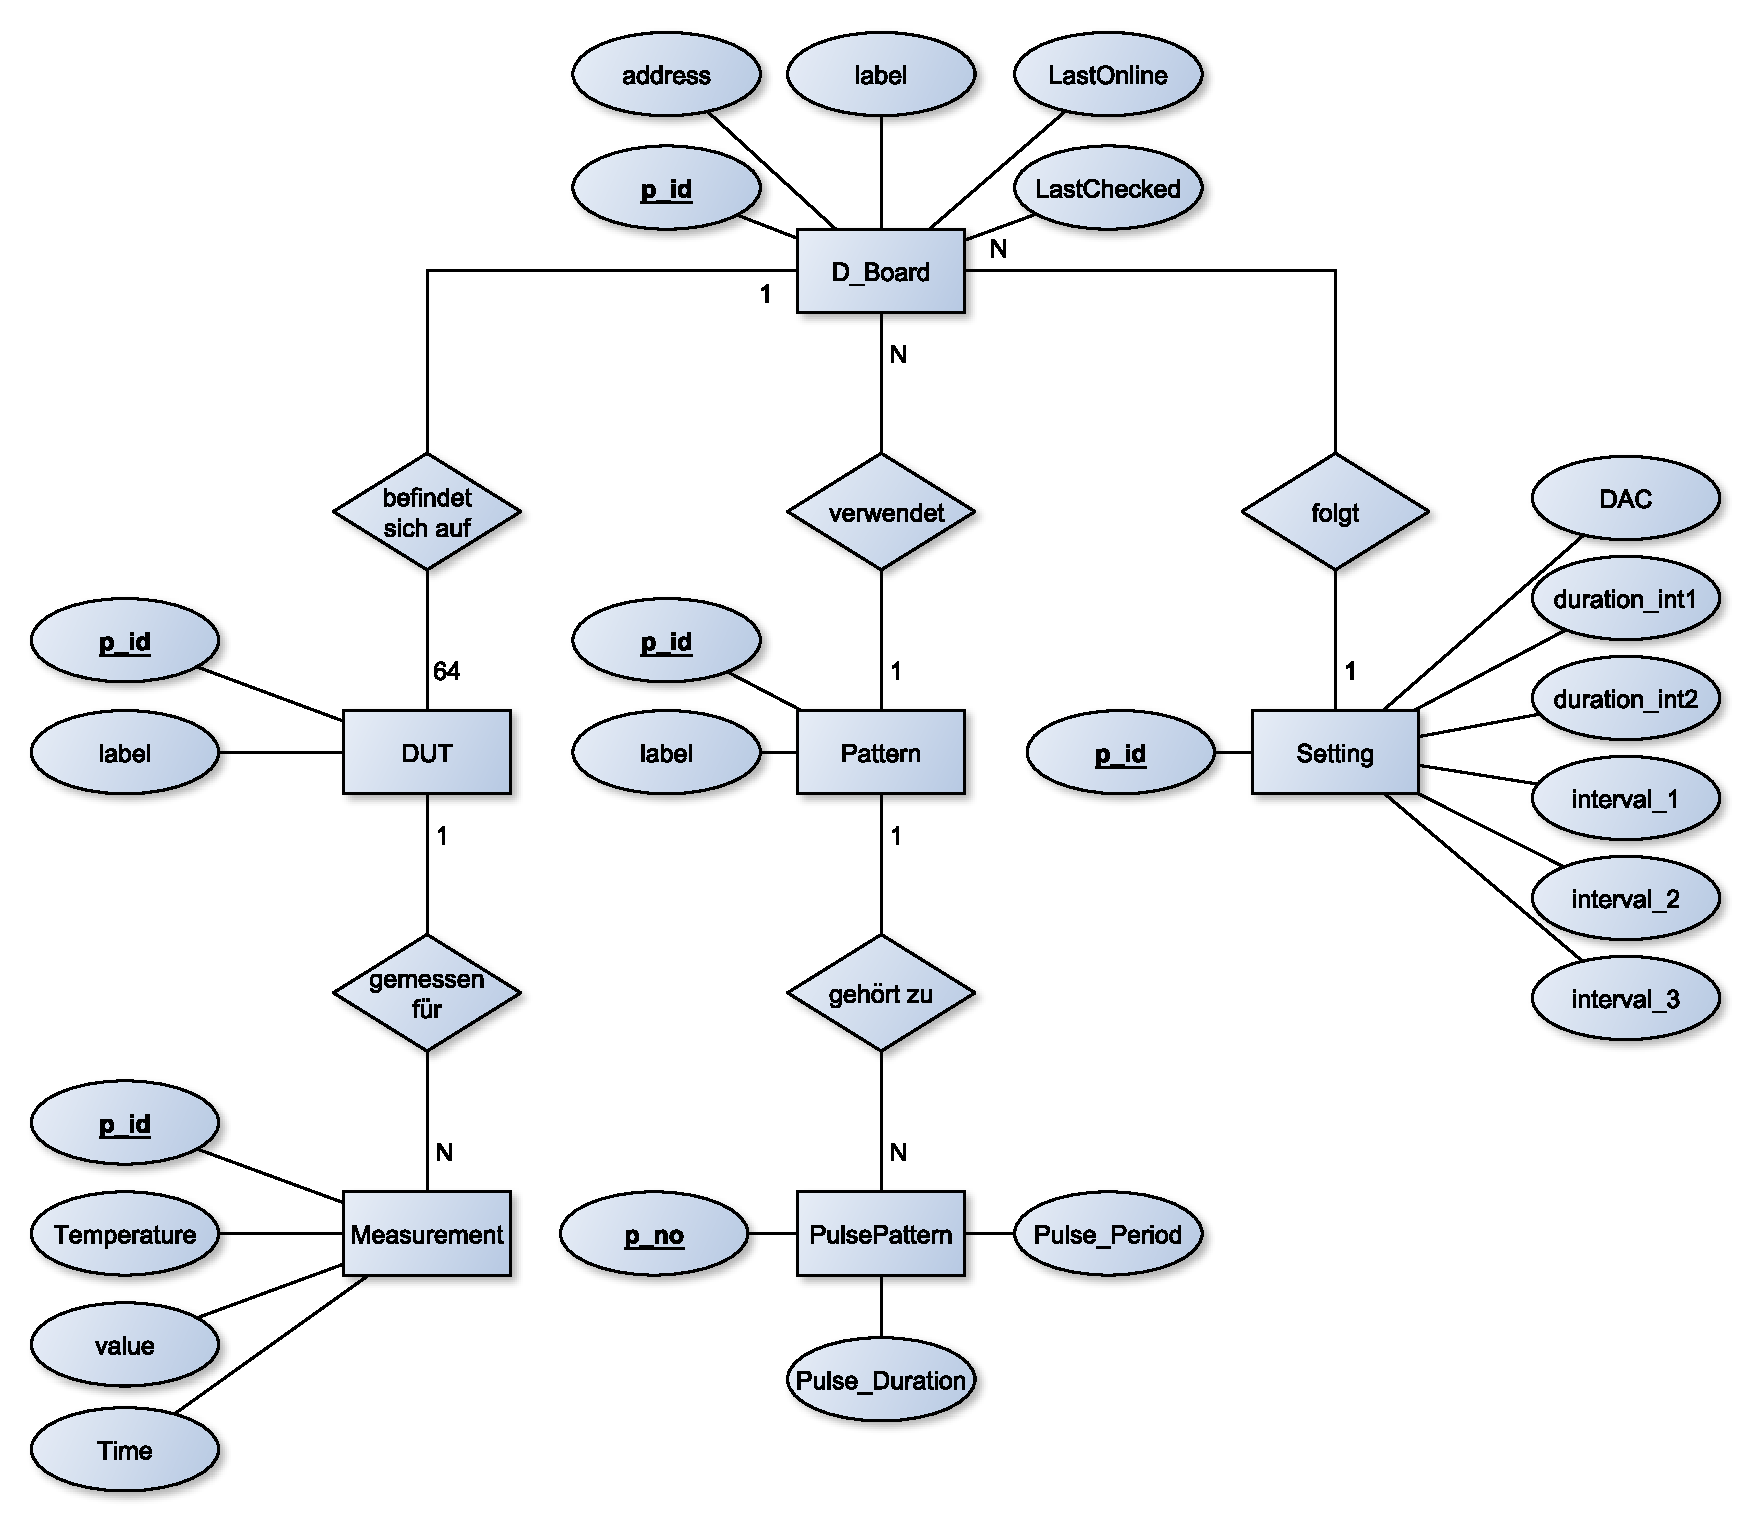
\includegraphics[width=\textwidth]{img/general/ER_Diagramm.pdf}
\caption{Entity Relationship Modell}
\label{ERM}
\end{center}
\end{figure}
